\chapter{ER-Diagram}\label{appendix:ER}
Our ER-diagrams follows a convention ER-convention. Each relation has a name,
and is intended to be read either from left to right or top towards bottom.

\begin{figure}[h!]
	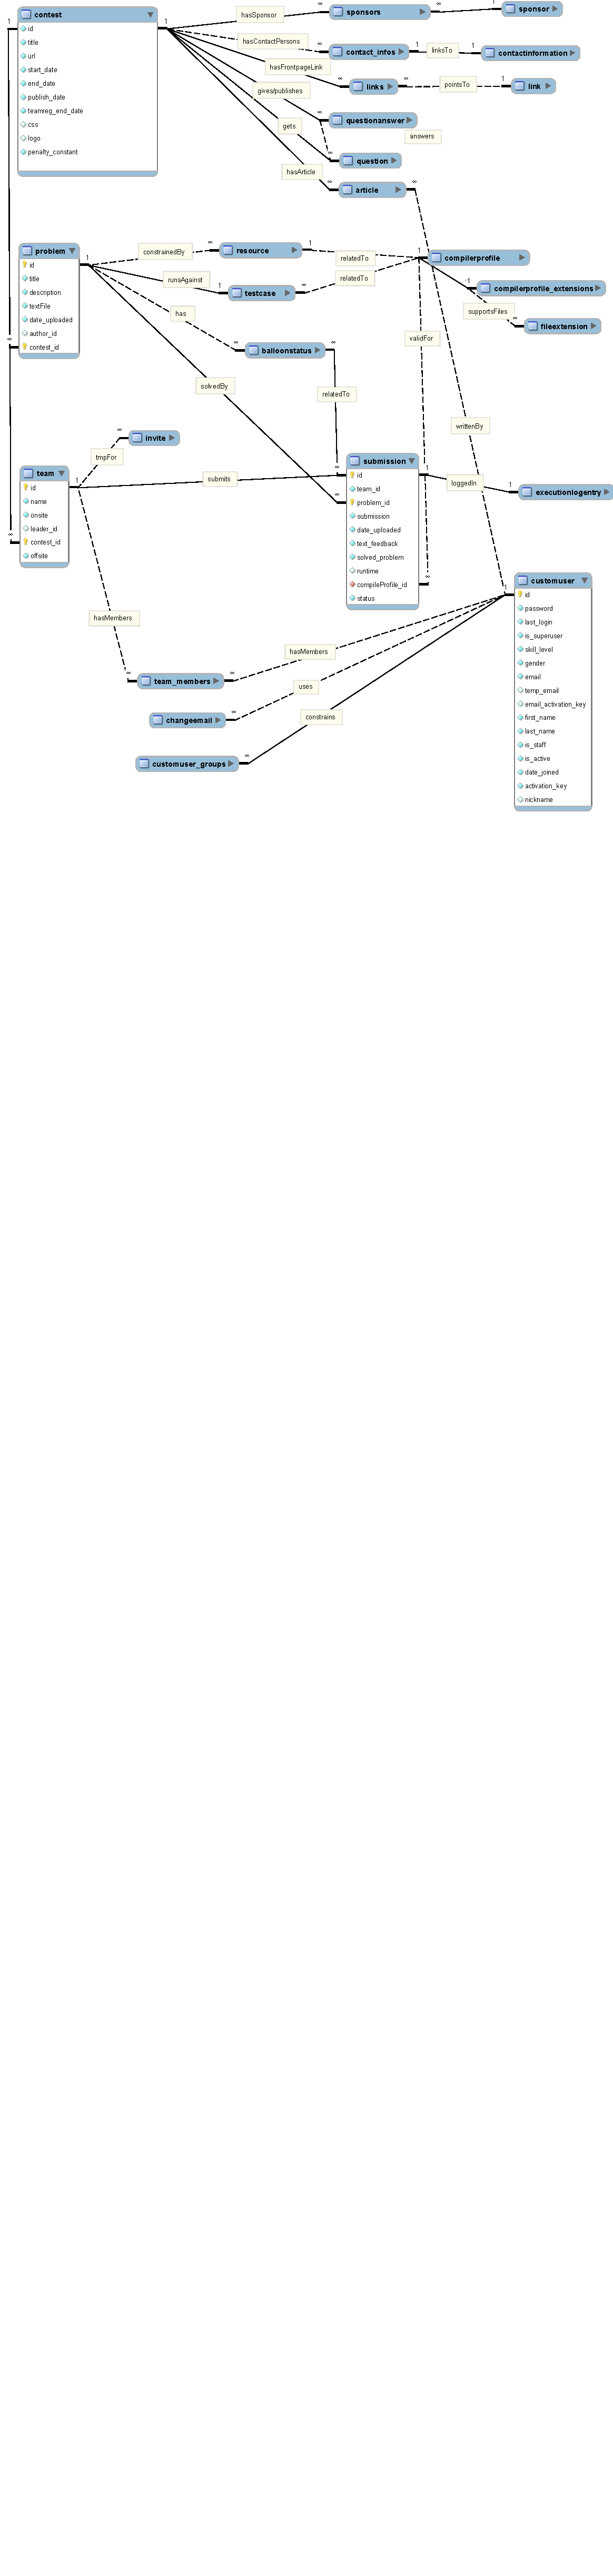
\includegraphics[scale=.65]{ER_complete.pdf}
	\caption{Complete ER-diagram. The un-folded classes are the main components
    of the system}
	\label{fig:ERComplete}
\end{figure}

\begin{figure}[h!]
	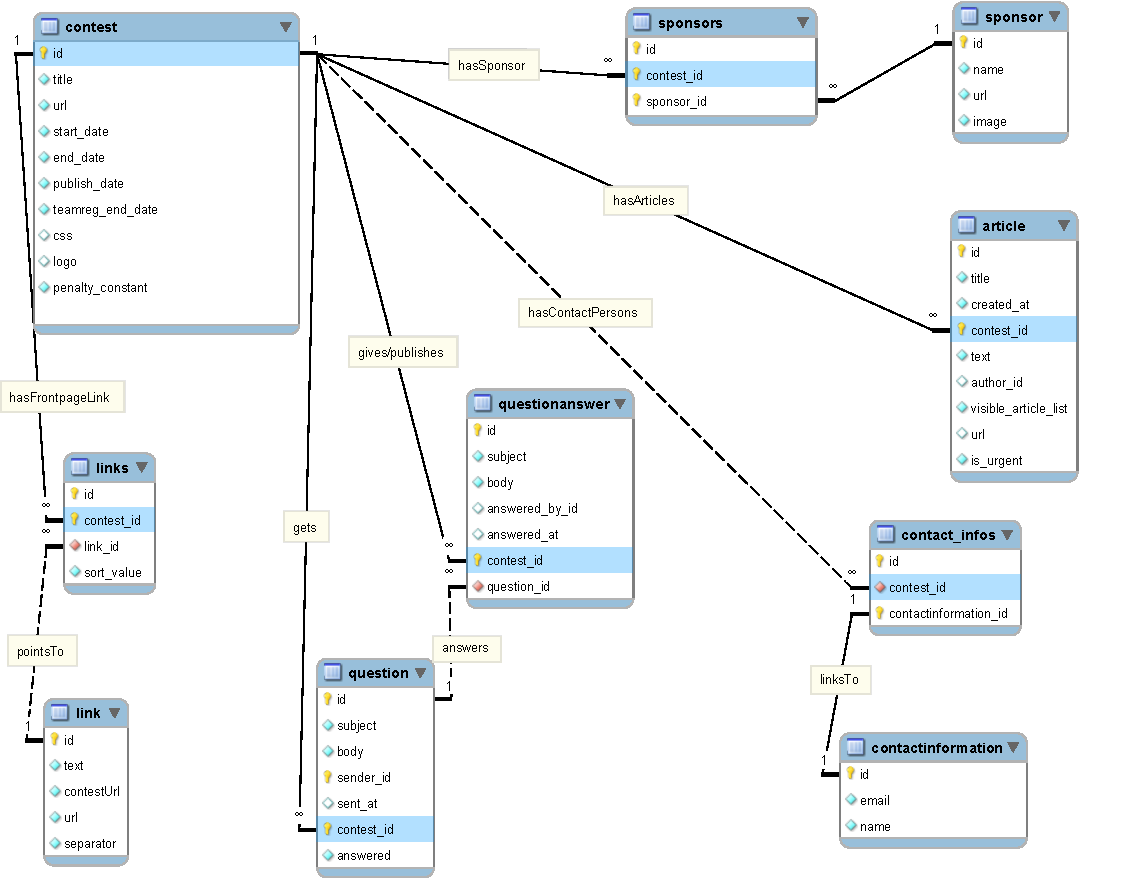
\includegraphics[scale=.65]{ER_contest}
    \caption{ER-diagram for the models used for the contest.}
	\label{fig:ERContest}
\end{figure}

\begin{figure}[h!]
	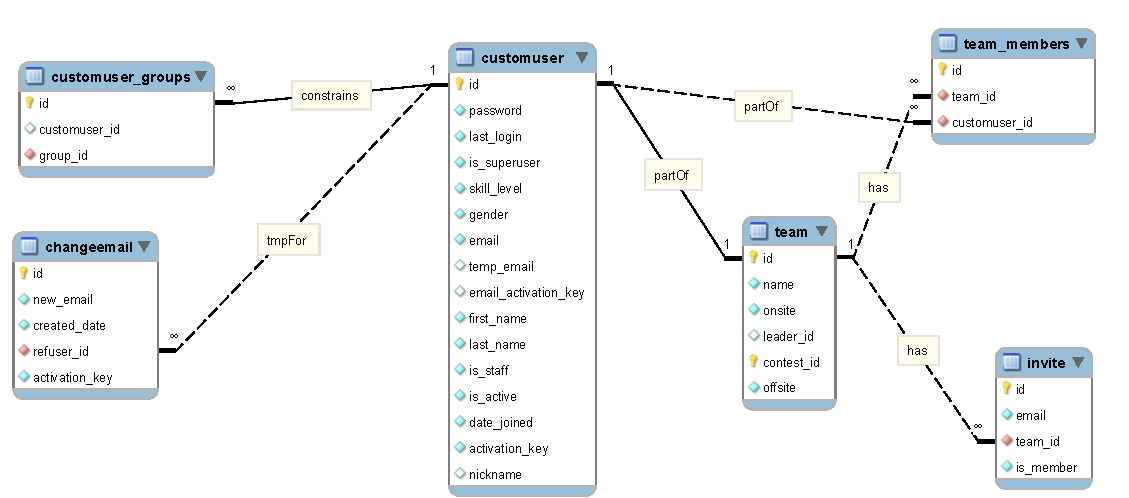
\includegraphics[scale=.65]{ER_customuser}
    \caption{ER-diagram for the models used for the user registration.}
	\label{fig:ERCustomuser}
\end{figure}

\begin{figure}[h!]
	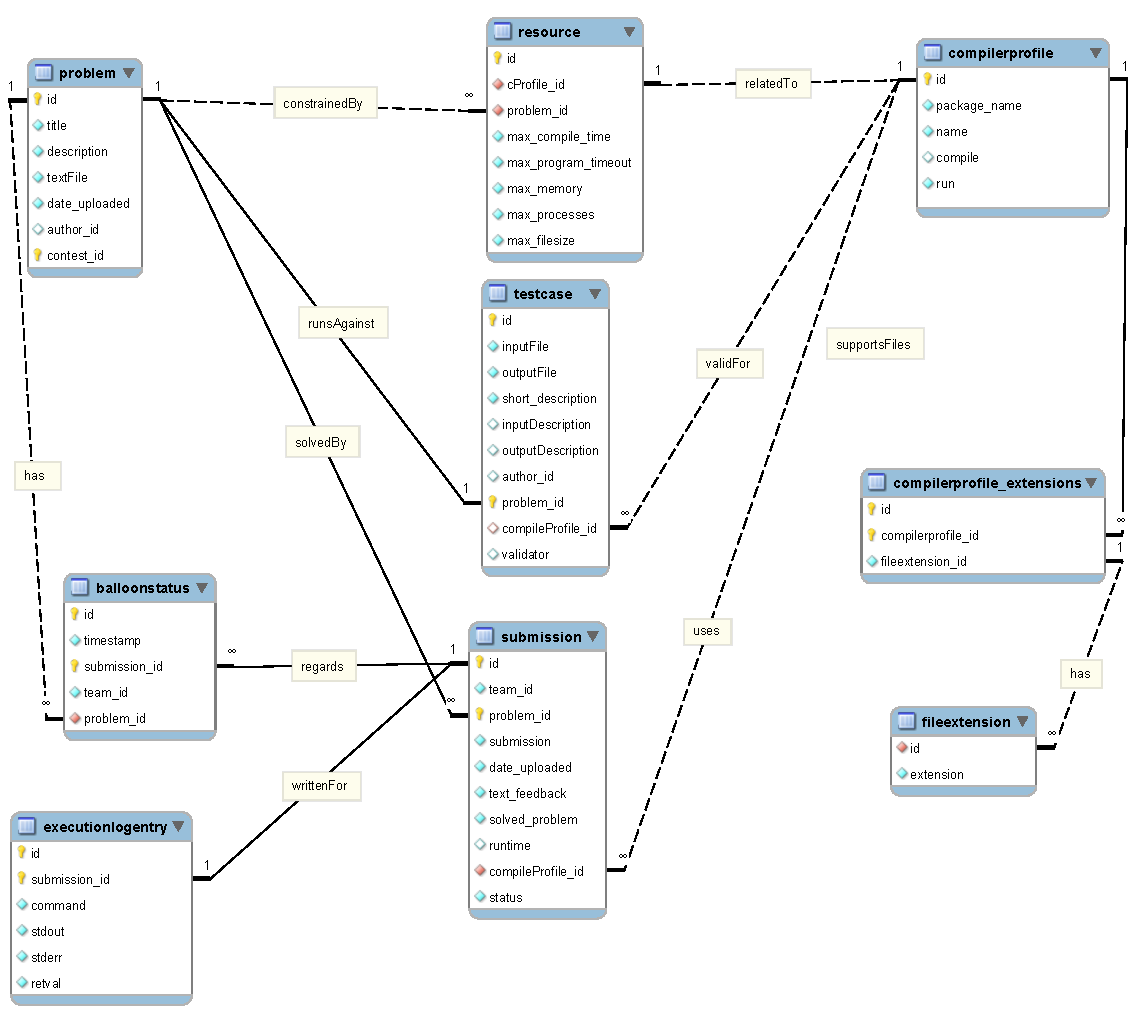
\includegraphics[scale=.65]{ER_submission}
    \caption{ER-diagram for the models used for the submission.}
	\label{fig:ERSubmission}
\end{figure}
